%-------------------------
% Resume in Latex
% Author : Matty
% Based on: https://github.com/jakegut/resume (which was itself based on https://github.com/sb2nov/resume)
% License : MIT
%------------------------

\documentclass[letterpaper,11pt]{article}

\usepackage{latexsym}
\usepackage[empty]{fullpage}
\usepackage{titlesec}
\usepackage{marvosym}
\usepackage[usenames,dvipsnames]{color}
\usepackage{verbatim}
\usepackage{enumitem}
\usepackage[hidelinks]{hyperref}
\usepackage{fancyhdr}
\usepackage[english]{babel}
\usepackage{tabularx}
\usepackage{xcolor}
\usepackage{fontawesome5}
\usepackage{graphicx}

\input{glyphtounicode}

% -------------------- FONT OPTIONS --------------------
% sans-serif
% \usepackage[sfdefault]{roboto}
% \usepackage[sfdefault]{noto-sans}
% serif
% \usepackage{charter}

\pagestyle{fancy}
\fancyhf{} % clear all header and footer fields
\fancyfoot{}
\renewcommand{\headrulewidth}{0pt}
\renewcommand{\footrulewidth}{0pt}

% Adjust margins
\addtolength{\oddsidemargin}{-0.5in}
\addtolength{\evensidemargin}{-0.5in}
\addtolength{\textwidth}{1in}
\addtolength{\topmargin}{-1in} % Default was -.5in
\addtolength{\textheight}{1.0in}

\urlstyle{same}

\raggedbottom
\raggedright
\setlength{\tabcolsep}{0in}

% Section formatting
\titleformat{\section}{
  \vspace{-5pt}\scshape\raggedright\large
}{}{0em}{}[\color{black}\titlerule \vspace{-5pt}]

% Subsection formatting
\titleformat{\subsection}{
  \vspace{-4pt}\scshape\raggedright\large
}{\hspace{-.15in}}{0em}{}[\color{black}\vspace{-8pt}]

% Ensure that generate pdf is machine readable/ATS parsable
\pdfgentounicode=1

% -------------------- CUSTOM COMMANDS --------------------
\newcommand{\resumeItem}[1]{
  \item\small{
    {#1 \vspace{-2pt}}
  }
}

\newcommand{\resumeSubheading}[4]{
  \vspace{-2pt}\item
    \begin{tabular*}{0.97\textwidth}[t]{l@{\extracolsep{\fill}}r}
      \textbf{#1} & #2 \\
      \textit{\small#3} & \textit{\small #4} \\
    \end{tabular*}\vspace{-7pt}
}

\newcommand{\resumeSubSubheading}[2]{
    \item
    \begin{tabular*}{0.97\textwidth}{l@{\extracolsep{\fill}}r}
      \textit{\small#1} & \textit{\small #2} \\
    \end{tabular*}\vspace{-7pt}
}

\newcommand{\resumeProjectHeading}[2]{
    \item
    \begin{tabular*}{0.97\textwidth}{l@{\extracolsep{\fill}}r}
      \small#1 & #2 \\
    \end{tabular*}\vspace{-7pt}
}

\newcommand{\resumeSubItem}[1]{\resumeItem{#1}\vspace{-4pt}}
\newcommand{\resumeSubHeadingListStart}{\begin{itemize}[leftmargin=0.15in, label={}]}
\newcommand{\resumeSubHeadingListEnd}{\end{itemize}}
\newcommand{\resumeItemListStart}{\begin{itemize}}
\newcommand{\resumeItemListEnd}{\end{itemize}\vspace{-5pt}}

\renewcommand\labelitemii{$\vcenter{\hbox{\tiny$\bullet$}}$}

\setlength{\footskip}{4.08003pt}

% -------------------- START OF DOCUMENT --------------------
\begin{document}

% Add graphicx package to the preamble

% -------------------- HEADING --------------------
\begin{flushright}
  % \vspace{-4pt}
  \color{gray}
  \item
  % Last Updated on January 12th, 2024
\end{flushright}

\vspace{-32pt}

\begin{center}
    \begin{minipage}{0.2\textwidth}
        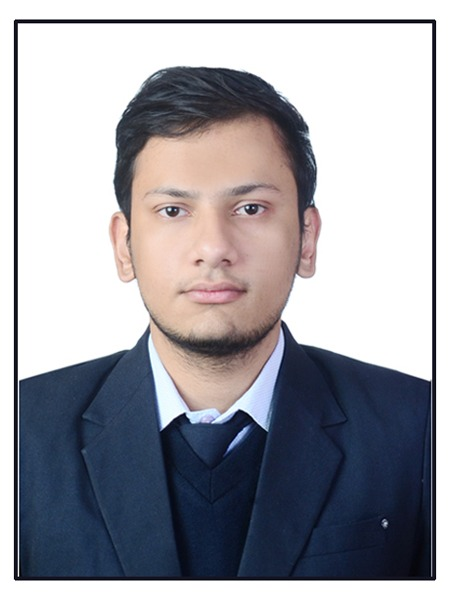
\includegraphics[width=\linewidth, height=1.2in, keepaspectratio]{IMG-20240412-WA0001.jpg}
    \end{minipage}%
    \begin{minipage}{0.80\textwidth}
        \textbf{\Huge \scshape Abhishek Tiwari} \\[5pt]
        \small 
        \faIcon{phone}
        \href{tel:626-8393-044}
        {\underline{626-8393-044}} $  $
        \faIcon{github}
        \href{https://github.com/Itz-Abhishek-Tiwari}{\underline{Itz-Abhishek-Tiwari}} $  $
        \faIcon{linkedin}
        \href{https://www.linkedin.com/in/itz-abhishek-tiwari/}{\underline{itz-abhishek-tiwari}} $  $
        \faIcon{envelope}
        \href{mailto:abhitiwariabhi7@gmail.com}
        {\underline{abhitiwariabhi7@gmail.com}} \\
        %\faIcon{map-marker-alt}
        %\href{https://g.co/kgs/AgNBcui}
        %{\underline{Indore, India}}
    \end{minipage}
\end{center}


% -------------------- Summary --------------------
% \section{Summary}

% \begin{itemize}[leftmargin=0.15in, label={}]
%     \text{I'm seeking a challenging role where I can leverage my web development experience and collaborative skills to drive innovation and contribute to organizational success while continuously improving my technical and communication abilities.}
    
% \end{itemize}


% -------------------- SKILLS --------------------
\section{\textbf{Skills}}
 \begin{itemize}[leftmargin=0.15in, label={}]
    \small{\item{
    
     \textbf{Languages}{: Python, JavaScript, SQL, HTML, CSS \vspace{4pt}} \\
     
     \textbf{Framework \& Library}{: Django, React, TailwindCSS, Bootstrap  \vspace{4pt}}\\
     
     \textbf{Miscellaneous Technology}{: Git/GitHub, Linux Shell}
     
     % \textbf{Frameworks}{: React, Node.js, Flask, JUnit, WordPress, Material-UI, FastAPI} \\
     
     % \textbf{Libraries}{: pandas, NumPy, Matplotlib}
     
    }}
 \end{itemize}
\vspace{0px}

 
% -------------------- EXPERIENCE --------------------
\section{\textbf{Experience}}
  \resumeSubHeadingListStart
          \resumeProjectHeading
          {\textbf{Front End Developer Intern} $|$ \footnotesize{Salesqueen Software Solutions}\vspace{4pt}}{Feb 2023 - Mar 2023}
           \resumeItemListStart
          {\resumeItem{Resolved a critical bug in an HR management dashboard, correcting issues with inaccurate graph rendering using ReactJS.}}
          {\resumeItem{Developed and implemented sub-tabs for employee login/logout records and upcoming leave dates with HTML and Bootstrap.}}
          {\resumeItem{Enhanced dashboard functionality by integrating additional features for improved HR management, leveraging ReactJS and Bootstrap for a responsive design.}}
          \resumeItemListEnd        
          \resumeSubHeadingListEnd

\vspace{0px}

% -------------------- PROJECTS --------------------
\section{\textbf{Projects}}
    \resumeSubHeadingListStart

        \resumeProjectHeading
       {\textbf{{BlogCraft}} $|$ \footnotesize{JavaScript, ReactJS, Python, Django,SQLite, Git}\vspace{4pt}}{}
        \resumeItemListStart
            \resumeItem{\textbf{User Roles \& Permissions:} Implemented a flexible system with distinct user roles and permissions for enhanced content management.}
            \resumeItem{\textbf{Markdown Support: }Integrated Markdown support for enriched post formatting and customization.}
            \resumeItem{\textbf{Data Export:} Enabled export of posts and comments to CSV and PDF formats for easy data management.}
          \resumeItemListEnd
    \vspace{4px}

        \resumeProjectHeading
        {\textbf{NoteMaster: Document Management System} $|$ \footnotesize{JavaScript, React.js, TailwindCSS, Git, Python, Django, SQLite}\vspace{4pt}}{}
        \resumeItemListStart
            \resumeItem{\textbf{User Authentication and Authorization:} Implemented secure user login, registration, and session management.}
            \resumeItem{\textbf{Search Functionality:} Implemented search features for easy retrieval of documents and notes.}
            \resumeItem{\textbf{Rich Text Editor:} Integrated a rich text editor using Slate.js for creating and editing documents with various formatting options.}
            \resumeItem{\textbf{Responsive Design:} Ensured the application is mobile-friendly with a responsive design using CSS and React.
}
          \resumeItemListEnd
          
      % \resumeProjectHeading
      %   {\textbf{FoodDropper} $|$ \footnotesize{Java, Maven, API (Spigot), Git, IntelliJ IDEA}}{Aug. 2022}
      %   \resumeItemListStart
      %       \resumeItem{Developed a Minecraft server plugin to limit players to one way of replenishing their hunger bar}
      %       \resumeItem{Used persistent data containers to save and load data, ensuring that it persists across plugin resets}
      %       \resumeItem{Optimized UX e.g. sound design, food drop timing, supplied saturation level, and addressed potential workarounds}
      %   \resumeItemListEnd

          
    \resumeSubHeadingListEnd

\vspace{0px}

% -------------------- EDUCATION --------------------
\section{\textbf{Education}}
  \resumeSubHeadingListStart
  
    \resumeSubheading
      {Shivajirao Kadam Institute Of Technology And Management, Indore}{JUNE 2020 - JUNE 2024}
      {B.Tech Computer Science}
      {CGPA: 8.07}
      {}
      
    \resumeSubheading
      {Aradhana higher secondary school, Neemuch}{APR 2019 - APR 2020}
      {Grade - XII}
      % {Neemuch}

      \resumeSubheading
      {Alpha higher secondary school, Neemuch}{APR 2016 - APR 2017}
      {Grade - X}
      % {Neemuch}

  \vspace{1px}

  \resumeSubHeadingListEnd


  \vspace{-2px}
% ------------------- Other accomplishments --------------------
\section{\textbf{Other accomplishments}}
  \resumeSubHeadingListStart

          \resumeProjectHeading
          {\textbf{Sports}\vspace{8pt}}{}
          {\small{Represented School Cricket Team as a Bowler for Team Secure, achieving 1st place in November 2020.}}

          \resumeProjectHeading
          {\textbf{Academic/Co-curricular Activities}\vspace{8pt}}{}
          {\small{Participated in the Science Fair at GEETANJALI INSTITUTE OF TECHNICAL STUDIES, UDAIPUR, where my team secured the Runner-Up position in December 2019.}}
          
    \resumeSubHeadingListEnd 
  \vspace{0px}


  

\end{document}
